\documentclass[a4paper]{article}
\usepackage{fullpage}
\usepackage[utf8]{inputenc}
\usepackage{graphicx}
\begin{document}
\section{Parser-Modul}
\textbf{Bitte berücksichtigen: Es kann noch Änderungen hieran geben, da dies nur eine Präsentation des aktuellen Standes ist...}
\subsection{Funktionalität}
Das Parser-Modul liest den gegebenen Assembler-Code,
führt alle gegebenen Compiler-Direktiven aus und generiert für jedes Argument einen Syntax-Baum,
der an die Architektur übergeben wird.
Außerdem reserviert er den über die Reservierungs- und Definierungsdirektiven festgelegten Speicher.

Somit entspricht der Parser dem Assemblierer.
Die Trennung von Architektur und Parser wurde vorgenommen,
um Code-Duplikation zu vermeiden,
die bei Architekturen mit mehreren Dialekten auftreten könnten (bei X86 z.B. AT\&T- und Intel-Syntax).
\subsection{Umsetzung (Referenzmodul)}
Das Referenzmodul (welches im Rahmen dieses Großpraktikums konstruiert werden soll) wird als bekannter 2-Pass-Assembler realisiert. Wie die Architektur wird dieses vorerst auf RISC-V (und hier einen bestimmten Dialekt) ausgelegt und spezialisiert sein.
\subsubsection{Entfernen von Kommentaren}
Zuvor werden alle Kommentare entfernt. Dieser Schritt ist nur notwendig, falls der RISC-V-Assembler mehrzeilige Kommentare unterstützen soll.
\subsubsection{1. Pass}
Im ersten Schritt wird der rohe Assemblertext gelesen und in Zeilenbereiche unterteilt, die jeweils einen Befehl mit allen zugehörigen Marken beinhalten.
Diese Befehle werden anschließend in Objekte gepackt (mit Zeilenintervall und Datei des Auftretens), wobei wir zwischen Direktiven und den eigentlichen Befehlen unterscheiden.
Besonders bei ersteren wird bereits hier genauer unterschieden.
Alle Labels und eventuell auch Konstantennamen (die wie Labels behandelt werden) werden in die Symboltabelle mit ihrem korrespondierenden (Text-)Wert geschrieben.
Wenn von Core oder GUI gewünscht (also wenn das Programm gerade nicht läuft), wird hier der Speicher reserviert, sonst werden nur die entsprechenden Positionen berechnet.
Bei allen Makros wird Anfang und Ende erfasst und diese in eine separate Makroliste eingetragen.
\subsubsection{2. Pass}
Wir haben nun eine Befehlsfolge von Objekten. In diesem Schritt werden nun die Direktiven ausgeführt und die Labels mit ihrem Wert eingesetzt.
Aus jedem der Argumente wird ein Syntaxbaum gebildet. Wegen möglichen unbekannten Datentypen anderer ISAs usw. wird hier eine Factory für Knoten vom Architektur-Modul bereitgestellt.
Als Ausgabe dient schließlich eine Liste von Objekten \emph{ohne} jegliche Direktiven und mit Argumenten als Syntaxbäumen. Diese wird dann dem Core zur Verfügung gestellt.
\begin{figure}
\centering
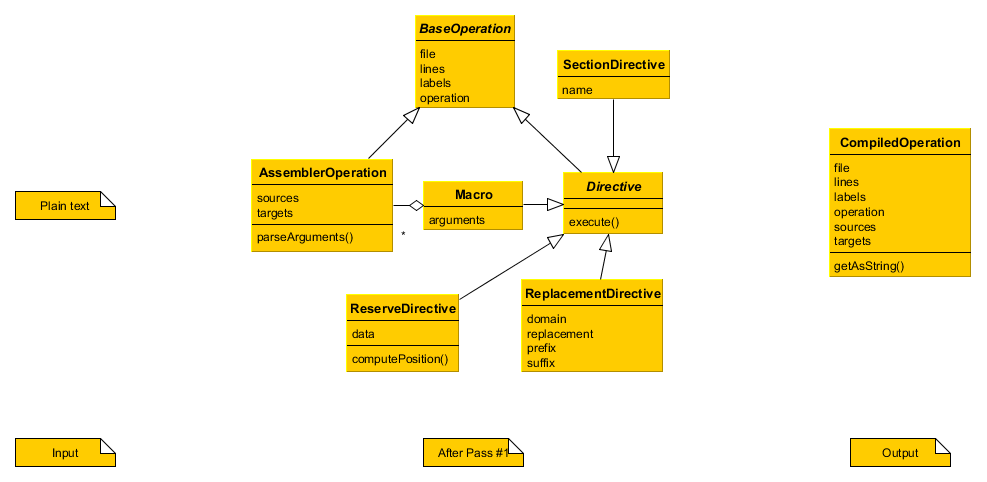
\includegraphics[width=0.8\textwidth]{process.png}
\caption{Eine grobe Skizze des Parsing-Prozesses.}
\end{figure}
\subsubsection{Geplante Direktiven-Unterstützung}
Unterstützt werden sollen:
\begin{itemize}
\item Makros
\item Speicherreservierungs- und Speicherbelegungs-Direktiven (z.B. resb, dd)
\item Konstantendefinitionen und Aliase (z.B. für Register)
\item Data-/Text-Sektion-Umschaltung
\end{itemize}
\emph{Nicht} unterstützt werden sollen:
\begin{itemize}
\item Bedingte Assemblerkompilierung
\item Komplett freie Textersetzungssysteme (z.B. C-Präprozessor)
\item Inkludieren anderer Assembler-Dateien
\end{itemize}
\subsection{Abhängigkeiten}
Der Parser kommuniziert mit allen anderen Modulen über den Core und ist somit alleine von diesem abhängig. 
Die Architektur erfragt vom Parser die einzelnen assemblierten Zeilen, um diese auszuführen.
Die GUI erhält vom Parser die Fehlermeldungen und stellt die Anfragen, um Code zu übersetzen.

Wir haben uns dazu entschieden, vorerst die boost::spirit-Bibliothek zu verwenden, um Ausdrücke zu parsen.
Wir erachten dies als sinnvoll, um das Projekt in Anbetracht der Stärke des Parser-Teams (zwei Personen) und der verfügbaren Zeit ordentlich fertigstellen zu können.
\subsection{Verworfen: Allgemeiner Parser}
Im Laufe unserer Entscheidungsfindung stand auch kurz auf dem Plan, einen allgemeinen Parser mit einem kleinen dialektabhängigen Modul zu entwerfen.
Dies hätte den Vorteil, dass die Dialektmodule wesentlich kleiner und einfacher zu programmieren ausgefallen wären, da die Hauptarbeit ja sowieso der große allgemeine Parser übernimmt.
Jedoch haben wir diese Idee für dieses Großpraktikum verworfen, da hierbei zu viele Komplikationen entstanden (wie will man fast alle Assemblersprachen verallgemeinern?).
Sie steht jedoch für spätere Projekte frei, verwendet zu werden.
\end{document}